\documentclass[11pt,a4paper]{article}
\usepackage[utf8]{inputenc}
\usepackage[english,catalan]{babel}
\usepackage{droid}
\usepackage[pdftex, pdfborderstyle={/S/U/W 0}]{hyperref} % this disables the boxes around links
\usepackage[pdftex]{graphicx}
\urlstyle{tt}

\author{
  Delicado Alcántara, Luis
  \\
  Conejo Micó, Xavier
  \\
  Sanchez Ferreres, Josep
}
\title{\Huge {Intel·ligència artificial}\\\medskip \huge{Treball sobre innovació:\\ - Cry Translator -}}

\begin{document}

\begin{titlepage}
\clearpage\maketitle
\thispagestyle{empty}
\end{titlepage}

\clearpage

\tableofcontents

\newpage

\section[\textsf{Què és Cry Translator?}]{\textsf{Descripció de producte: Què és cry translator?}}
\label{quees}

Cry Translator \cite{official} és un aparell que permet identificar el motiu del plor d'un nadó. Aquest producte està disponible en tres versions: Un aparell amb forma de \emph{walkie-talkie} (figura \ref{fig:walkie}), integrat en un peluix\footnote{Tot i que la pàgina web oficial no menciona la versió en peluix, la pàgina web de biloop si que en parla. Sospitem que hi ha una incoherència entre les dues pàgines webs deguda a una desactualització. El fet que hagin esborrat material respecte aquesta versió del producte també ens porta a sospitar que encara no està llesta o van escollir retirar-la del mercat.} (figura \ref{fig:peluix}) o disponible en una aplicació d'iOS. 

Cry Translator és un producte desenvolupat per Biloop Technologic S.L., i un dels seus principals clams és que el seu producte ha estat provat clínicament \cite{estudi_clinic} i que té un nivell de fiabilitat del 96\% \cite{official} \cite{elmundo}. 

El funcionament de l'aparell és senzill. En les tres versions del producte n'hi ha prou amb acostar l'aparell entre 20cm i 1m del nadó plorant, i el propi aparell ens indicarà, en un lapse curt de temps\footnote{3s per l'aparell dedicat i fins a 10s per l'aplicació d'iPhone} quin és el motiu del plor del nadó classificat en 5 categories diferents: son, estrés, gana, descomfort i avorriment.

Per recolzar la seva credibilitat, cry translator ha desenvolupat d'un únic estudi clínic (\cite{estudi_clinic}) a més de diverses opinions d'experts i premsa totes accessibles desde la pàgina oficial.

\begin{figure}[hb]
\centering
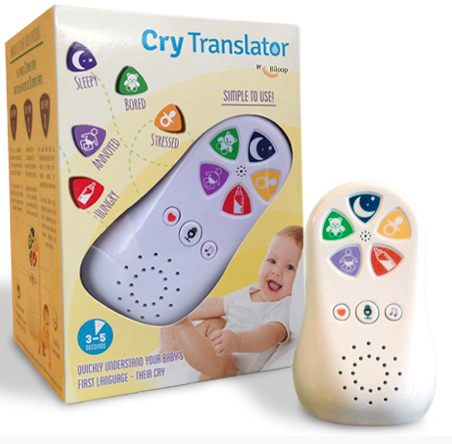
\includegraphics[width=0.5\textwidth]{./fig/walkie.png}
\caption{Cry translator en la seva versio \emph{walkie-talkie}}
\label{fig:walkie}
\end{figure}

\begin{figure}[ht]
\centering

\includegraphics[width=0.5\textwidth]{./fig/peluix.png}
\caption{Cry translator en la seva versio peluix}
\label{fig:peluix}
\end{figure}

\section{\textsf{Tècniques d'IA utilitzades en el producte}}
\label{tecniques}

Cercant per diverses fonts, principalment \cite{patent} i \cite{elmundo}, hem pogut establir que aquesta aplicació utilitza un algoritme de lògica difusa. A continguació en els següents apartats es justifica que la tècnica utilitzada es correspon a un camp de l'intel·ligència artificial i expliquem breument el funcionament.

\subsection{\textsf{Descripció de les tècniques utilitzades}}
\label{descripcio}

Com s'explica posteriorment amb més detall a l'apartat \ref{us-tecniques}, Cry Translator fa servir un algorisme de lògica difusa per fer el filtrat de les senyals. En aquest apartat veiem com la lògica difusa és una eina matemàtica utilitzada abastament en la intel·ligència artificial i quin paper juga en el filtrat de senyals.

La lògica difusa és un model de lògica que permet tractar amb coneixement imperfecte i/o incomplet. A diferència dels sistemes basats en regles que hem utilitzat a l'assignatura un sistema basat en lògica difusa és, doncs, capaç de lidiar amb aquest tipus de coneixement. Veiem com ja d'entrada és adecuat parlar de coneixement imprecís quan parlem d'anàlisi de senyals, i aquest fet s'accentua si els aparells de mesura son tan imperfectes com els que pugui tenir un telèfon mòbil.

Per tal de modelar aquesta imprecisió, els predicats de lògica difusa no tenen valor binari de cert o fals, sinó que tenen un valor continu des de 0, o totalment fals, fins a 1, o totalment cert. 

Però com s'aplica aquest model al processament de senyals? Com s'explica a \cite{fuzzy}, la lògica difusa és juntament a les xarxes neuronals artificials, un dels mètodes més utilitzats en l'àmbit del processament de senyals amb un fort component de soroll. Queda fora de l'àmbit d'aquest document una explicació completa de com utilitzar tècniques de lògica difusa al processament de senyals. No obstant s'intenta donar una idea intuitiva per convencer-nos que aquesta tècnica és aplicable.

Per a donar una idea del paper de la lògica difusa en el processament de senyals vegem un dels sistemes més emprats, els sistemes de lògica difusa de tipus 1 (o TLS, tal com se'ls anomena a \cite{fuzzy}). A la figura \ref{fig:tls-1}\footnote{Aquesta figura ha estat extreta del document original (\cite{fuzzy}) i tot el crèdit per aquesta és de l'autor original} podem veure l'esquema bàsic d'un TLS de tipus 1. Aquest sistema, tal com es veu intenta mapejar entrades a sortides. En el context de Cry Translator, com veurem més endavant, l'entrada es correspon al plor del nadó i la sortida a quina de les senyals predefinides s'assembla més. 

L'esquema bàsic de la figura \ref{fig:tls-1} és molt semblant al d'un sistema clàssic basat en regles. Per una banda tenim les regles, que representen el coneixement de l'expert, i que son processades pel motor d'inferència per tal de fer deduccions a partir dels predicats de lògica que es donin com a entrada. 

La diferència princial recau en el funcionament del motor d'inferència, i de manera indirecta en la manera d'especificar les regles. Això es deu al fet que aquestes venen donades pel \emph{Fuzzifier}, que converteix les senyals d'entrada a predicats de lògica difusa. Així doncs podem imaginar-nos que els algoritmes del motor d'inferència seràn notablement diferents als d'un motor d'inferència de lògica clàssica. També podem veure que la manera d'especificar les regles serà diferent. En aquest cas diversos predicats, aparentment contradictoris en un context de lògica clàssica, poden ser parcialment certs o falsos a la vegada.

Per últim cal comentar que aquest procés de raonament necesita un pas final de refinament, per convertir els predicats de lògica difusa en valors de veritat (i.e. cert o fals), aquesta tasca correspon a l'element \emph{Defuzzifier} del sistema.

Vist el funcionament i capacitats d'aquest sistema, no és difícil convèncer-nos que els diversos valors d'una senyal es poden convertir en predicats de lògica difusa. Com veiem a la figura \ref{fig:calor}, posant l'exemple més senzill d'una temperatura, veiem com el predicat \emph{calor} pot ser parcialment cert al mateix temps que el de \emph{tebi}. Aplicant un raonament similar podriem atribuir valors als diveros valors mesurats d'una senyal. Per exemple: ``És 0.5-cert que aquesta senyal magnètica té una amplitud de tantes unitats'' és un exemple de possible predicat amb el qual pot treballar el TLS de reconeixement de senyals.

Tot i no donar una explicació completa del processament de senyals mitjançant lògica difusa, queda vist que aquesta és aplicable en aquest camp i és una tècnica molt utilitzada d'intel·ligència artificial pel reconeixement de patrons.

\begin{figure}[hbt]
\centering
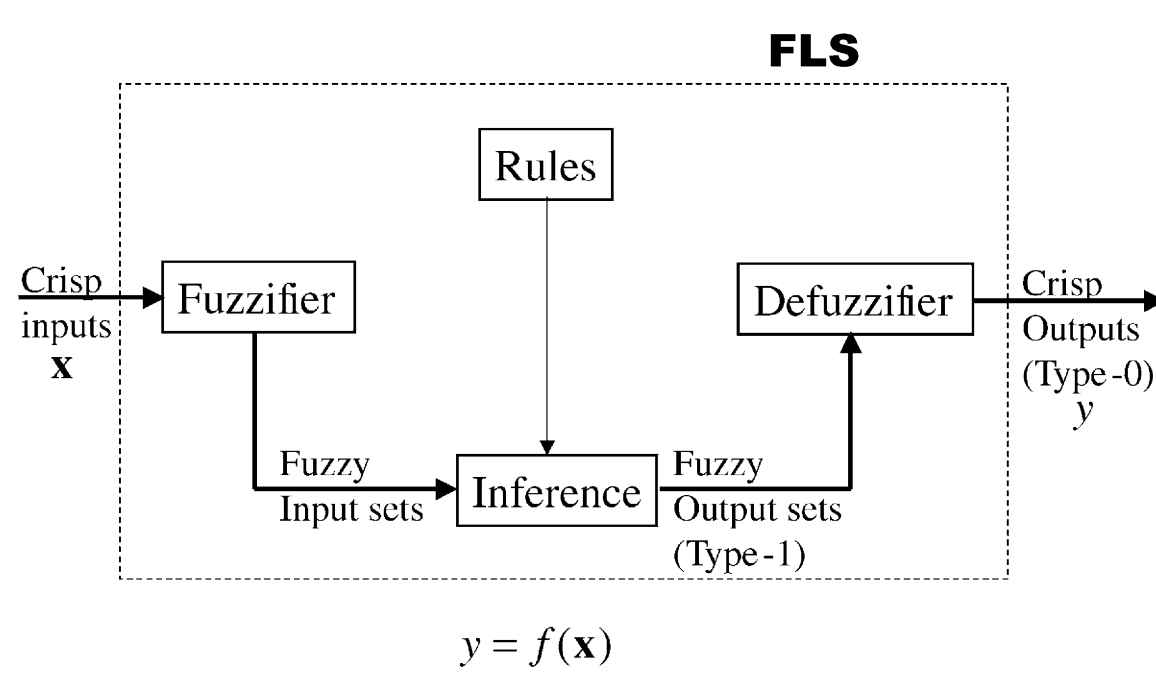
\includegraphics[width=0.8\textwidth]{./fig/tls1.png}
\caption{Esquema bàsic t'un TLS de tipus 1}
\label{fig:tls-1}
\end{figure}

\begin{figure}[hbt]
\centering
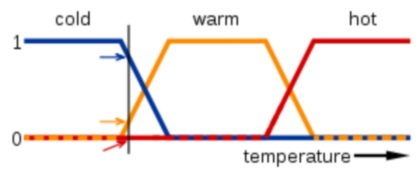
\includegraphics[width=0.7\textwidth]{./fig/fuzzy.png}
\caption{Gràfic de valors de lògica difusa per diferents valors de temperatura.}
\label{fig:calor}
\end{figure}
\clearpage


\subsection{\textsf{Ús de les tècniques per a l'implementació del producte}}
\label{us-tecniques}

L'algoritme de lògica difusa que es fa servir no queda massa clar ni tan sols a la patent del producte \cite{patent}. I cal destacar que hem realitzat nombrosos intents de contactar amb els creadors del producte sense resposta. No obstant hem extret tota l'informació que hem pogut per tal d'explicar en quin context es fa servir i quina tasca es resol amb l'algoritme.

En primer lloc cal destacar que l'objectiu del producte és permetre mesurar la senyal provinent del plor d'un nadó a una distància d'entre 20cm i 1m de distància.

L'objectiu del producte, de manera més tècnica, consisteix en l'anàlisi de senyals periòdiques en un context d'un microcontrolador de baix pressupost. Veiem com aquest és també el cas d'un mòbil, ja que encara que els processadors dels mòbils siguin cada cop més potents, les seves capacitats de mesura de senyals electromagnètiques a través d'un micròfon segueixen sent bastant limitades.

El que s'intenta fer és analitzar l'amplitud de la senyal fent un reconeixement de l'ona del sò i ajustar aquest valor dins d'unes quantes senyals ``arquetip'', que en el cas de cry translator corresponen als diferents plors d'un nadó. Aquestes senyals s'han estudiat i modelat prèviament. Concretament de cada senyal es guarda:
\begin{itemize}
\item Mitjana de les dades, i de l'arrel quadrada i del quadrat d'aquestes
\item \emph{Work cycle} de la senyal (ratio entre la durada del pols i el periòde de la senyal)
\item Primera i segona derivades de la senyal
\item Màxim i mínim
\end{itemize}
Tots aquests valors s'han calculat prèviament i emmagatzemat en unes matrius de referència corresponent a diferents tipus de plors de nadons. El programa intentarà classificar la matriu calculada com una de les matrius guardades prèviament. Veiem doncs que el programa no disposa de cap capacitat d'aprenentatge. També veiem que ja d'entrada el podem considerar un sistema basat en el coneixement que utilitza informació provinent de sensors.

El paper de la inteligència artificial, però, va més enllà. És evident que la senyal que Biloop va mesurar en un laboratori serà només remotament semblant a la que es pugui mesurar amb tot el soroll de l'entorn a més de la mala qualitat del sistema que capta la senyal. A part, aquesta senyal es troba resumida en uns quants indicadors estadístics, cosa que complica encara més el reconeixement, ja que no es disposa de la senyal original. És per això que resulta necessari un algoritme que permeti filtrar tot aquest soroll i fer el reconeixement de patrons en les senyals que permeti classificar-les en els diferents tipus de plors de nadons. Aquest mateix sistema també es pot fer servir per tal de mesurar altres tipus de patrons en la veu, com l'estat d'ànim d'una persona adulta, tal com s'indica a \cite{patent}.

Així doncs, l'algoritme de lògica difusa s'empra per filtrar la senyal i fer un \emph{pattern matching} entre els valors de la senyal mesurada i els valors de referència de les matrius. Gràcies a aquest algoritme que es pot dur a terme aquesta tasca de filtrat i reconeixement de senyals amb un hardware tan rudimentari com és el micròfon d'un telèfon mòbil, o un microcontrolador de propòsit general de baix pressupost. Veiem doncs que el paper de les tècniques d'intel·ligència artificial és crucial en l'implementació d'aquesta aplicació.

Queda vist, doncs, com cry translator utilitza la intel·ligència artificial i perquè podem dir que és un producte basat en aquest camp.

\section{\textsf{Riscos i beneficis de l'innovació}}
\label{riscos-beneficis}

\subsection{\textsf{Per què Cry translator és un producte innovador?}}
\label{justificacio}

\subsection{\textsf{Impacte del producte en l'empresa}}
\label{impacte-empresa}

\subsection{\textsf{Impacte del producte en la societat}}
\label{impacte-societat}

\clearpage
\begin{thebibliography}{1}

\bibitem{official} Cry translator, pàgina oficial

Disponible a: \url{http://www.crytranslator.com/en/}

\bibitem{fuzzy} Jerry M. Mendel, \emph{Uncertainty, fuzzy logic, and signal processing}

Disponible a: \url{http://sipi.usc.edu/~mendel/publications/Mendel%20SP%202000.pdf}

\bibitem{patent} Juan Pedro Barrera Vazquez, et. al., \emph{Signal Recognition Method With a Low-Cost Microcontroller}. 

Disponible a: \url{http://www.faqs.org/patents/app/20080284409}

\bibitem{elmundo} Elena Soto, per a El Mundo (Diari), \emph{Un oído que traduce el llanto del bebé}

Disponible a: \url{http://www.elmundo.es/elmundo/2009/12/28/baleares/1262020419.html}

\bibitem{estudi_clinic} Portugal Ramírez, A., \emph{Uso del Cry Translator de Biloop Technologic S.L. (España) como identificador del llanto en el niño y pautas a seguir }

Disponible a: \url{http://www.crytranslator.com/images/expertos/Estudio\_Clinico.pdf}

\bibitem{expert} Ellen Abell, \emph{Infant Crying: ``I’m Trying To Tell You Something!''}

Disponible a: \url{http://www.crytranslator.com/images/expertos/Alabama\_Cooperative\_Extension\_System.pdf}
\end{thebibliography}

\end{document}